%%
%% Meta: Master Document
%% TALS Funktionen I
%%

%% So kann die Größe für alle Skripts direkt verändert werden
\documentclass[twoside,14pt,a5paper]{extarticle}

\usepackage{bbw}

\renewcommand{\author}{Philipp G. Freimann}
\renewcommand{\grafikautor}{Ph. G. Freimann}
\renewcommand{\authoremail}{philipp.freimann@bbw.ch}
\renewcommand{\erstellungsdatum}{28. Nov. 2021}
\renewcommand{\docversion}{1.8.0(\LaTeX{})}

%%\renewcommand{\modulnummer}{Arithmetik und Algebra I}
\renewcommand{\doctitel}{Funktionen 1}
\renewcommand{\fachthema}{lineare Funktionen}


%%%%%%%%%%%%%%%%%%%%%%%%%%%%%%%%%%%%%%%%%%%%%%%%%%%%%%%%%%%%%%%%%%%%

\begin{document}
\newcommand{\linkGressLy}{\spancode{http://www.gress.ly/oo/oo.pdf}}%%
\newcommand{\linkLiskov}{\spancode{http://www.pmg.csail.mit.edu/\textasciitilde{}liskov/}}%%
\newcommand{\linkProgrammierenlernenCh}{\spancode{http://www.programmieraufgaben.ch}}%%
\newcommand{\linkProgrammierenlernenChOO}{\spancode{http://www.programmieraufgaben.ch/uploads/oo.pdf}}%%
\newcommand{\linkWikiSingleton}{\spancode{http://de.wikipedia.org/wiki/Singleton\_(Entwurfsmuster)}}%%
\newcommand{\linkWikiDesignPattern}{\spancode{http://de.wikipedia.org/wiki/Entwurfsmuster}}%%

\newcommand{\linkVerzeichnis}{%%
%%\newpage%%
\section{Link-Verzeichnis}\index{Linkverzeichnis}%%
Verzeichnis aller verwendeten Links aus den vorangehenden Kapiteln.
\begin{itemize}%%
 \item \linkGressLy{}: Download zu diesem Buch
 \item \linkLiskov{}: Polymorphismus: Das Substitutionsprinzip
 \item \linkProgrammierenlernenCh{}: Aufgabenbuch zu diesem Skript
 \item \linkProgrammierenlernenChOO{}: Download zu diesem Buch
 \item \linkWikiSingleton{}: \textit{Singleton}-Pattern
 \item \linkWikiDesignPattern{}: Entwurfsmuster (\textit{Design-Pattern})
\end{itemize}%%
}%%


\ptitlepage
\newpage

%% Arithmetik und Algebra Grundlagen
%%
%% TALS Metapackeg Funktionen IV

%%%%%%%%%%%%%%%%
\part{Funktionen IV}\index{Funktionen!IV|textbf}
%%
%% 2019 07 04 Ph. G. Freimann
%%

\section{Wachstum und Zerfall}\index{Wachstum}\index{Zerfall}
\sectuntertitel{Sagt ein großer Stift zum kleinen Stift: ``Wachsmalstift!''}
%%%%%%%%%%%%%%%%%%%%%%%%%%%%%%%%%%%%%%%%%%%%%%%%%%%%%%%%%%%%%%%%%%%%%%%%%%%%%%%%%
\TRAINER{Video Mathe Mann}%%
\subsection*{Lernziele}

\begin{itemize}
\item Zinseszins
\item Wachstums-, Zerfallsprozesse
\item Verdoppelungs- und Halbwertszeiten
\item Basiswechsel
\end{itemize}

\TALS{(\cite{frommenwiler17alg} S.221 (Kap. Exponentielles Wachstum))}
\TALS{(\cite{frommenwiler17alg} S.223 (Kap. Exponentielle Abnahme))}
\TALS{(\cite{frommenwiler17alg} S.225 (Kap. Zinseszins))}
\GESO{(\cite{marthaler17}       S.342 (Kap. 20))}


\subsection{Beispiele}
Bei ungebremsten Prozessen sprechen wir dann von einer exponentieller
Zunahme, wenn die Zunahme pro Zeiteinheit jeweils proportional zur aktuellen Anzahl ist.

\begin{itemize}
\item \Lueckentext{Zinseszins}
\item \Lueckentext{Frequenzen in der temperierten Stimmung (Musik). Zunahme der Frequenz pro Halbtonschritt.}
\item \Lueckentext{Keime in der Kuhmilch; Ansteckungsbedingte Krankheitsfälle (\zB viral)}
\item \Lueckentext{Algenbefall in Teichen}
\item \Lueckentext{(ungebremstes) Bevölkerungswachstum / bzw. Tierpopulation}
\item \Lueckentext{\dotfill}
\end{itemize}

\begin{bemerkung}{}{}
Oft wird bei Wachstumsprozessen die Zeitachse auch mit $t$ statt $x$ bezeichnet $t$ steht für \textit{time}.
\end{bemerkung}
\newpage

\subsection{Einstiegsbeispiel Zinseszins}
Skizzieren Sie ein Vermögen von CHF 10\,000.-, wie es  innerhalb
von zehn Jahren bei gleichbleibendem Zinssatz von 5\% verändert.


($y$-Achse in 10\,000.- CHF)


\bbwGraph{-1}{11}{-1}{3}{
\TRAINER{  \bbwFuncC{pow(1.05,\x)}{0:10}{blue}
}%% end TRAINER
}%% end graph

\newpage
\begin{definition}{Exponentialfunktion}{}\index{Exponentialfunktion!Definition}
  Eine Funktion der Form $$f(x): x \mapsto a^x$$
  bzw. $$y = a^x$$
  heißt \textbf{Exponentialfunktion}.
\end{definition}

Zeichnen Sie $f: y=2^x$ und $g: y=1.4^x$ ins selbe Koordinatensystem:


\bbwGraph{-5}{5}{-1}{5}{
\TRAINER{  \bbwFuncC{pow(2.0,\x)}{-3.5:2.1}{blue}
  \bbwFuncC{pow(1.4,\x)}{-3.5:3}{green}
  \bbwLetter{1,3}{$f$}{blue}
  \bbwLetter{2.5,2}{$g$}{green}
}%% end TRAINER
}%% end graph



\begin{bemerkung}{Wachstumsfaktor}{}\index{Wachstumsfaktor}
Der Parameter $a$ gibt den Wachstumsfaktor pro Zeiteinheit $e_x$ an.
\end{bemerkung}

\newpage

\subsection{Allgemeine Form der Exponentialfunktion}

Obige Exponentialfunktion hat für den Wert $x=0$ immer den $y$-Wert = 1. Da dies in der Praxis aber meist nicht der Fall ist, gib es die folgende \textbf{allgemeine Form der Exponentialfunktion}:

\begin{definition}{allgemeine Exponentialfunktion}{}
$$f: y = b\cdot{}a^x$$

Auch hier gibt der Parameter $a$ den Wachstumsfaktor pro Zeiteinheit $e_x$ an.

Dabei ist $b$ der Startwert zum Zeitpunkt $x$ = 0.
\end{definition}


\bbwCenterGraphic{8cm}{allg/funktionen/img/exp/b_faktor.png}

\begin{bemerkung}{Wachstumsfaktor}{}{}
Werden zwei $x$ Positionen mit Differenz 1 (=$e_x$) betrachtet, so sind
die zugehörige $y$-Werte um \textbf{Faktor} $a$ auseinander.
\end{bemerkung}

Begründung:
\TNT{4}{
  Gegeben $x_1$ und $x_2 = x_1 + 1$. So ist

  $y_1 = b\cdot{}a^{x_1}$ und $y_2 = b\cdot{}a^{x_2}$.

  Setzen wir nun $x_1 + 1$ für $x_2$ ein, so erhalten wir:

  $$y_2 = b\cdot{} a^{x_1+1} = b\cdot{}a^{x_1}\cdot{}a^1 = a\cdot{}b\cdot{}a^{x_1} = a\cdot{}y_1$$
}
\newpage



\subsection{Einstiegsbeispiel}
Der Türlersee ist ein kleiner See im Repischtal. Seine Oberfläche
begann sich vor einigen Jahrzehnten stark mit Algen\footnote{Genau
  genommen handelte es sich um Zooplanktonbiomasse zwischen 1982 und 1994, doch als
  Idee zur Exponentialfunktion soll das Flächenmodell reichen.} zu bedecken.

Anfänglich (zum Zeitpunkt $t=0$) waren gerade mal 20$m^2$ bedeckt. Doch nach fünf Tagen hatte sich diese Fläche verdoppelt und nach weiteren fünf Tagen nochmals verdoppelt (also insgesamt vervierfacht).

Füllen Sie die (prognostizierte) Wertetabelle für 30 Tage ein:

\def\spaceX{\,\,\,\,\,\,\,\,\,\,}
\newcommand\tuerlerB[1]{\noTRAINER{\spaceX}\TRAINER{#1}}
\begin{tabular}{l|c|c|c|c|c|c|c}
  $t$:  & 0 & 5 & 10 & 15 & 20 & 25 & 30 \\
  \hline
  $m^2$ & \tuerlerB{20}  & \tuerlerB{40}  &   \tuerlerB{80}  &  \tuerlerB{160}  &  \tuerlerB{320}  &  \tuerlerB{640}  &  \tuerlerB{1280} \\
\end{tabular}


Zeichnen Sie die Algenpopulation als Graph in eine Koordinatensystem
(beginnen Sie mit dem Ursprung ganz links unten. Eine $x$-Einheit,
also ein Tag,  nach rechts entspricht einem Häuschen und in $y$-Richtung nehmen Sie 2 Häuschen für 100$m^2$ Algenfläche:

\TNT{11.2}{\bbwGraphic{10cm}{allg/funktionen/img/tuerlerAlgen.png}}

Geben Sie eine Funktionsgleichung an, welche das Wachstum der Algenpopulation beschreibt:

\begin{center}
  $f:\,\,\, y=\LoesungsRaumLang{20\cdot{} 2 ^{\frac{t}{5}}}$
  \end{center}
\TRAINER{
Dabei bezeichnet 20 den Startwert, 2 den Zunahmefaktor und 5 die Beobachtungszeitspanne.}%%

\newpage



\subsubsection{Grundform}

Die allgemeine Formel für exponentielle Prozesse lautet:

\begin{definition}{Wachstumsprozess}{}
  $$f(t) = y = b\cdot{}a^{\frac{t}{\tau}}$$
\end{definition}

\subsubsection{Graphische Erläuterung}

\bbwCenterGraphic{11cm}{allg/funktionen/img/exp/exponentielles_wachstum.png}


Dabei sind
\begin{itemize}
\item $b=f(0)$ der Anfangsbestand zum Zeitpunkt $t$ = 0.
\item $\tau$ ist die typische Zeitspanne zwischen zwei Beobachtungszeitpunkten (zum Beispiel zwischen Wert und dessen Verdopplung). Beispiele:
  \begin{itemize}
  \item Verdoppeln in 3 Stunden: $a=2$ und $\tau = 3 [\textrm{h}]$
  \item Verfünffachen einer Viertelstunde (= 15 Minuten): $a=5$ und
    $\tau=\frac{1}{4} [\textrm{h}]$
  \end{itemize}
\item $a$ ist der Zunahmefaktor zwischen zwei Beobachtungszeitpunkten (Beispiel $a=2$ bei Verdoppelungsprozessen).
  $a$ berechnet sich durch den Quotienten zwischen zwei Beobachtungswerten $b$ und später $m$. Also $a=\frac{m}b=\frac{f(\tau)}{f(0)}$.
\item $f(t)=b\cdot{}a^{\frac{t}{\tau}}$ ist der Wert (Anzahl, Fläche,
  Bestand, ...) zum Zeitpunkt
  $t$. 
\end{itemize}

Bemerkung: 
\TNT{2.4}{
$\frac{f(\tau)}{f(0)}=\frac{b\cdot{}a^{\frac{t}{\tau}}}{b\cdot{}a^{\frac0{\tau}}}
  = a^{\frac{t}{\tau} -\frac{0}{\tau}} = a^{\frac{t-0}{\tau}}
  = a^{\frac{\tau}{\tau}} = a$}%% END TNT

\newpage

\subsection{Referenzaufgabe}\index{Irland!Bevölkerungswachstum}
Irland hatte 1990 3.5 Mio. Einwohner. Im Jahr 2019 waren es bereits 4.9 Mio.

\textbf{Frage 1}: Was prognostizieren Sie für das Jahr 2025, wenn Sie von einem exponentiellen Wachstum ausgehen?

\TNT{12}{
  1. Skizze:Ersichtlich: $\tau$, 1990, 2019, 3.5 und 4.9 (Rest irrelevant)
  
  Ansatz: Zeitpunkt $t_1 = 1990$, somit $m_1 = 3.5$ (Mio.). Analog Zeitpunkt $t_2 = 2019$ somit $m_2 = 4.9$ (Mio).
  Das $\tau= 29$ Jahre und das zugehörige $a$ ist $\frac{4.9}{3.5}$. $a$ abspeichern!

  Uns fehlt noch das $b$.

  Es gilt nun im Jahr 1990 ($=t_1$): $3.5 = f(1990) = b\cdot{} \left(a\right)^\frac{t_1}{\tau} = b\cdot{} a^\frac{1990}{29}$

  Somit ist $$b = \frac{3.5}{  a^\frac{1990}{29}  } \approx 3.3\cdot{}10^{-10}$$

  Dieses Resultat $b$ abspeichern!

  Nun können wir die Prognose für 2025 einfach berechnen: $f(2025) = b\cdot{}a^\frac{2025}{29}$, denn wir haben ja $a$ und $b$ bereits im Rechner gespeichert.
}%% ENT TNT
\newpage

\textbf{Frage 2}: In wie vielen Jahren hat sich die Bevölkerung verdoppelt?

\TNT{12}{
  Halbwertszeit sei $T$. Ansatz: $a^\frac{t}{29} = 2^\frac{t}{T}$ und somit (auf beiden Seiten die $t$-te Wurzel:

  $a^\frac{1}{29} = 2^\frac{1}{T}$ (Nun beidseitig $\log_a$.)

  $\frac{1}{29} = \frac1T \cdot{}\log_a(2)$ (Nun den Kehrwert)

  $29 = T \cdot{} \frac{1}{\log_a(2)}$ (und noch mal $\log_a(2)$)

  $T = 29 \cdot{} \log_a(2) \approx 59$ Jahre
}%% END Trainer
\newpage

\subsection*{Aufgaben}
\TALSAadB{221ff}{831 - 839}
\GESOAadB{207}{10.}
\GESOAadB{338}{28. Bakterien}
\GESOAadB{352ff}{2., 7., 1. (optional)}
\GESO{\aufgabenfarbe{Kompendium: S. 27ff: 32., 34., 37., 38., 40., 44., 45. und 46.}}
\GESO{\aufgabenfarbe{Nullserie Aufgabe 8}}
\GESO{\aufgabenfarbe{Maturaprüfung 2017, Aufg. 12 (Raupen)\\
Maturaprüfung 2018 (Serie 3), Aufg. 11 (Müll)
}}

\newpage


\subsection{Exponentieller Zerfall}\label{zerfallsfunktion}
Die Funktion $f(t): t \mapsto y = d^{-t}$ ist eine
Exponentialfunktion, die gegen Null geht.
\bbwFunction{-4}{4}{-1}{8}{exp(-\x)}{-2:4}

\newpage

\subsubsection{Beispiele}
\begin{itemize}
	\item \Lueckentext{Zinsliche Abschreibungen (\zB Wert eines Autos)}
	\item \Lueckentext{Radioaktiver Zerfall}
	\item \Lueckentext{Lichtintensität in Medium (Gas / Flüssigkeit / Glasfaser), dies gilt vertikal, wie auch horizontal}
	\item \Lueckentext{Atmosphärischer Luftdruck in Metern über Meer}
  \item \Lueckentext{Entladen einer Batterie bzw. eines Kondensators}
  \item \Lueckentext{Sauerstoffkonzentration in Seen (\zB Herbst bei kontinuierlicher Abnahme)}
  \item \Lueckentext{Abnahme des Bierschaums im Glas}
  \item \Lueckentext{Mischen, wie im Sirup-Beispiel\totalref{sirup_beispiel}}
  \item \Lueckentext{«Halbwertszeit des Wissens» ;-)}
  \item \Lueckentext{\dotfill}
\end{itemize}

\newpage



Zeichnen Sie die Funktionen $f: y=2^x$, $g: y=2^{-x}$ und $h: y=\left(\frac12\right)^x$ in dasselbe Koordinatensystem:

\bbwGraph{-6}{6}{-1}{5}{
  \TRAINER{\bbwFuncC{exp(0.69314718*\x)}{-6:2}{blue}}
  \TRAINER{\bbwFuncC{exp(-0.69314718*\x)}{-2:6}{red} }
  \TRAINER{\bbwLetter{1.5,4}{2^x}{blue}}
  \TRAINER{\bbwLetter{-3,4}{2^{-x}=\left(\frac{1}{2}\right)^x}{red}}
}
\newpage
Die allgemeine Formel für Zerfallsprozesse lautet:

\begin{definition}{Zerfall}{}
$$f(t) = y = b\cdot{}a^{\frac{t}{\tau}}$$
\end{definition}

\bbwCenterGraphic{10cm}{allg/funktionen/img/exp/exponentieller_zerfall.png}

Dabei sind
\begin{itemize}
\item $b$ der Anfangsbestand zum Zeitpunkt $t$ = 0.
\item $\tau$ ist die Zeitspanne zwischen zwei typischen Beobachtungszeitpunkten (Zum Beispiel zwischen Wert und dessen Halbierung).
\item $a=\frac{f(\tau)}{f(0)}$ ist der Abnahmefaktor ($0<a<1$) zwischen zwei Beobachtungszeitpunkten (im Abstand von $\tau$). Bei Halbierungsprozessen \zB wäre $a=0.5$.
\end{itemize}

\begin{bemerkung}{Wachstum vs. Zerfall}{}

  Der einzige Unterschied bei Wachstums- bzw Zerfallsprozessen ist der
  Faktor $a$:

  \begin{itemize}
  \item $a>1$: Wachstum
  \item $0<a<1$: Zerfall
    \end{itemize}
  
  \end{bemerkung}
\newpage

\subsubsection{Umkehrung (Optional)}
Anstelle eines  positiven Exponenten ($\frac{+t}{\tau}$) kann genauso
gut der Kehrwert des Faktors $a$ genommen werden. Dann wird der
Exponent negativ, dafür wird die Basis $> 1$. Seien $m_1$ bzw. $m_2$
zwei Beobachtungswerte.

Mit $a = \frac{m_2}{m_1}$ und $d := \frac{m_1}{m_2} = \frac{1}{a}$, gilt

\begin{center}
  \fbox{$b\cdot{} a^{\frac{+t}{\tau}} = b\cdot{}d^{\frac{-t}{\tau}} $}
\end{center}

\TALS{Beweis:}\GESO{Begründung: So gilt \zB bei Halbierungsprozessen, dass $a=0.5$ und $d=2$:}

\TALS{ $b\cdot{}a^{\frac{t}{\tau}} = b\cdot{} \left(\frac{m_2}{m_1}\right)^{\frac{t}{\tau}} = b\cdot{} \left(\frac{m_1}{m_2}\right)^{\frac{-t}{\tau}} =  b\cdot{}d^{\frac{-t}{\tau}} $}
\GESO{ $b\cdot{}0.5^{\frac{t}{\tau}} = b\cdot{} \left(\frac{1}{2}\right)^{\frac{t}{\tau}} = b\cdot{} \left(\frac{2}{1}\right)^{\frac{-t}{\tau}} =  b\cdot{}2^{\frac{-t}{\tau}} $}
\newpage

%% Sirup-Beispiel
\subsubsection{Mischtank}\index{Mischtank}\index{Sirup}\label{sirup_beispiel}
Wird ein Glas Wasser in ein Glas Sirup geschüttet, so

\TRAINER{\bbwCenterGraphic{5cm}{allg/alg/potenzen_wurzeln/img/Schwapp.png}}%%
\noTRAINER{\bbwCenterGraphic{5cm}{allg/alg/potenzen_wurzeln/img/SchwappOhneFormel.png}}

geschieht erst mal etwas eher klebriges:
\begin{itemize}
  \item Das Wasser verdrängt den Sirup und
  \item das Sirupglas schwappt über.
\end{itemize}

Wenn man nun gleichzeitig im Sirupglas
umrührt, so mischt sich das Wasser mit dem Sirup und je länger man
Wasser einschüttet, umso verdünnter wird der Sirup.


Wie viel Sirup bleibt im Glas?

\TNT{2.4}{
Am Ende bleibt ein
Verhältnis von Wasser : Sirup = $\left(1-\frac{1}{e}\right) : \left(\frac{1}{e}\right)$
\vspace{1.5cm}
}

Diese Konstante wird oft in großen chemischen Mischtanks verwendet,
gibt aber auch ein Maß an, wenn \zB in einer Minergie-Wohnung die Luft
ausgetauscht wird. Wenn nämlich das Volumen der Wohnung einmal neu hineingepumpt (bzw. weggeblasen) wurde während sich alte die Luft im Haus permanent mit der neuen vermischt, so ist noch ein Anteil von \TRAINER{$\frac{1}{e}$}\noTRAINER{ ..... } der alten Luft im Haus.
\newpage


\textbf{Begründung:}\\
1. Gedanke: Jedes eingefüllte Glas, vermindert die vorhandene
Sirupkonzentration um den selben Faktor. Ergo handelt es sich um
einen exponentiellen Zerfall.

\leserluft

2. Gedanke: Wir tauschen drei Mal $\frac13$ aus. Nehmen also im
\begin{itemize}
\item \textbf{ersten Schritt} $\frac13$ des Sirups weg (und ersetzen diesen mit Wasser).
  Es bleiben $\frac23$ Sirup. Den Rest füllen wir mit Wasser auf.
\item Im \textbf{zweiten Schritt} nehmen wir $\frac13$ des Gemisches
weg; es verbleiben also $\frac23$ von $\frac23$ an
Sirup-Konzentrat. Der Rest wird immer wieder mit Wasser aufgefüllt. Mit
anderen Worten: Es bleiben $\frac23 \cdot \frac23
= \left(\frac23\right)^2$ an Sirup\footnote{Man könnte hier auch argumentieren mit: «Wir nehmen von den $\frac23$ einen Drittel weg»: $\frac23 - (\frac13$ von $\frac23)$ = $\frac23 - (\frac13 \cdot\frac23) = \frac23 \cdot(1-\frac13)=\frac23\cdot\frac23$}.
\item Im \textbf{dritten Schritt} entnehmen wir wieder $\frac13$ des
Gemisches; es verbleiben wieder $\frac23$ vom bisherigen Sirup, also
$\frac23$ von $(\frac23)^2$ also $\left(\frac23\right)^3$.

Beim dreistufigen Gedankenexperiment verbleiben
$\left(\frac23\right)^3 = \left(1-\frac13\right)^3$ der ursprünglichen Konzentration.
\end{itemize}
\leserluft

3. Gedanke: Das Experiment vom vorherigen Gedanken können wir natürlich auch mit immer kleineren\TALS{, sogenannten infinitesimalen,} Schritten durchführen.
Mit Centilitern \zB im dl-Glas ersetzen wir 10 Mal je $\frac1{10}$. 
So verbleibt am Schluss $\left(1-\frac{1}{10}\right)^{10}\approx 0.35$ Sirup.

\GESO{Wenn wir (\zB mit dem Taschenrechner) die Schrittanzahl immer weiter vergrößern (und somit die pro Schritt ausgetauschte Menge immer verkleinern), so ergibt sich für 1000 Schritte ein Verhältnis von $\left(1-\frac{1}{1000}\right)^{1000}\approx 0.3677 \approx \frac1e$. }
\TALS{Wenn wir die Schritte permanent erhöhen (und gegen Unendlich gehen lassen), so erhalten wir den Grenzwert (lat. Limes) von

$$\lim_{n\rightarrow\infty} \left(1-\frac{1}{n}\right)^n = \frac1e$$
}
\newpage

\textbf{Aufgabe 1: Sirup}\\
Wie viel Wasser muss eingeschüttet werden, damit das auf der Flasche
angegebene Verhältnis von 1:6 (1 Teil Sirup, 6 Teile Wasser) zustande
kommt?

\TNT{8}{
Bei 1x Schütten, erhalten wir $\left(\frac{1}{e}\right)^1$ Anteil Sirup.

Bei 2x Schütten, erhalten wir $\left(\frac{1}{e}\right)^2$ Anteil Sirup.

Somit erhalten wir den Siebtel (1:6 = $\frac17$-Anteil) indem wir die
folgende Exponentialgleichung lösen:

$$\frac17 = \left(\frac{1}{e}\right)^n$$
Diese Gleichung lösen wir, indem wir beidseitig logarithmieren und so
erhalten wir den einzuschüttenden Teil $$n=\ln(7)\approx{1.946}.$$
}%% END TNT

\textbf{Aufgabe 2: Minerige-Haus}\\
Wenn wir also wissen wollen, wie viel Luft in ein Minergiehaus
eingepumpt werden muss, damit nur noch 1 Promille der alten Luft
vorhanden ist, so erhalten wir
\TNT{2.4}{
$$\textrm{Volumen Neuluft} = \textrm{Wohnungsvolumen}\cdot{}\ln(1000)$$
} %% end TNT


\newpage



\subsection*{Aufgaben}
\TALSAadB{223ff}{840-847}
\GESOAadB{338}{29. (Bierschaum)}
\GESOAadB{352ff}{3, 4, 5, 6}
\GESOAadB{354ff}{9. (Bauchspeicheldrüse)}
\GESO{\aufgabenfarbe{Kompendium S. 27ff Kap. 3.4.1 33., 35., 36., 39., 41. 42., 43. und 47}}
\GESO{\aufgabenfarbe{
    Maturaprüfung 2018 (Serie 4), Aufg 10 (Cäsium 137)\\
    Maturaprüfung 2018 (Serie 2), Aufg 11 (Plutonium)\\
    Maturaprüfung 2018 (Serie 1), Aufg 11 (radioaktive Substanz)\\
    Maturaprüfung 2016, Aufg. 9 (Jod-131)
}}

\newpage

\subsection{Halbwertszeit, Verdopplungszeit}\index{Halbwertszeit}\index{Verdopplungszeit}

Die Zeitspanne, in der sich eine Menge halbiert, nenne wir
\textbf{Halbwertszeit}\footnote{Die Halbwertszeit wird inbesondere
  beim radioaktiven Zerfall verwendet: nach wie viel tausend Jahren strahlt
  ein Stoff nur noch die Hälfte.}.

Aus $\frac12\cdot{}b = f(t_{0.5}) = b\cdot{}a^{\frac{t_{0.5}}{\tau}}$
folgt\TRAINER{ beidseitig durch $b$ teilen und dann $log_a$}:

\begin{gesetz}{Halbwertzszeit}{}
  $$t_{0.5} = \tau\cdot{}\log_a\left(\frac12\right)$$
\end{gesetz}

Beispiel: Ein Stoff nimmt innerhalb von sieben Tagen auf 80\% ab. Wie
groß ist seine Halbwertszeit $t_{0.5}$?

\TNT{5.2}{$\tau=7$ und $a = 0.8$. Somit
$$t_{0.5} = 7\cdot{} \log_{0.8}\left(\frac12\right)\approx 21.74
  [\textrm{Tage}]$$
\vspace{2cm}}


Analog gilt das Gesetz zur Verdopplung (s. obiges Beispiel Bevölkerung Irlands):
\begin{gesetz}{Verdopplungszeit}{}
  $$t_2 = \tau\cdot{}\log_a(2)$$
\end{gesetz}

\newpage
\newpage
%%
%% 2019 07 04 Ph. G. Freimann
%%

\section{Exponentialfunktionen}\index{Funktion!Exponentialfunktion}\index{Exponentialfunktionen}
\sectuntertitel{Go viral!}
%%%%%%%%%%%%%%%%%%%%%%%%%%%%%%%%%%%%%%%%%%%%%%%%%%%%%%%%%%%%%%%%%%%%%%%%%%%%%%%%%
\subsection*{Lernziele}

\begin{itemize}
\item Definition Exponentialfunktion
\item Koeffizienten interpretieren
\item Graph: Symmetrien, Polstellen, Asymptoten, Schnittpunkte mit Achsen
\end{itemize}

\TALS{(\cite{frommenwiler17alg} S.215 (Kap. 3.10))}
\GESO{(\cite{marthaler17}       S.322 (Kap. 19))}


%  Besser bei der Zins und Zinseszinsformel
%\subsection{Einstiegsbeispiel}
%
%(Einstiegscomics «Donald Duck» im OLAT)
%\newpage



\begin{definition}{Exponentialfunktion}{}\index{Exponentialfunktion!Definition}
  Eine Funktion der Form $$f(x): x \mapsto a^x$$
  bzw. $$y = a^x$$
  heißt \textbf{Exponentialfunktion}.
\end{definition}

Der Parameter $a$ gibt den Wachstumsfaktor pro Zeiteinheit $e_x$ an.
 Oft wird die Zeitachse auch mit $t$ statt $x$ bezeichnet $t$ steht für \textit{time}.
\newpage

\subsection{Allgemeine Form der Exponentialfunktion}

Obige Exponentialfunktion hat für den Wert $x=0$ immer den $y$-Wert = 1. Da dies in der Praxis aber meist nicht der Fall ist, gib es die folgende \textbf{allgemeine Form der Exponentialfunktion}:

\begin{center}\fbox{$f: y = b\cdot{}a^x$}\end{center}

Dabei ist $b$ der Startwert zum Zeitpunkt $x$ = 0.

\bbwCenterGraphic{8cm}{allg/funktionen/img/exp/b_faktor.png}
\newpage



\subsubsection{Verschiebung und Streckung}

Eine Verschiebung der Exponentialfunktion $y=b\cdot{}a^x$ in der Zeit ($x$-Richtung) kann auch in Form einer Veränderung der Startfaktors $b$ umgeschrieben werden.

Verschieben wir \zB $$y=2^x$$ um fünf Einheiten nach rechts, so liest sich die neue Funktionsgleichung wie folgt:
$$y=2^{x-5}.$$

(Zeichnen Sie in \texttt{geogebra.org} a) $y=2^x$ und b) $y=2^{x-5}$.)

Dies kann jedoch auch umgeschrieben werden:

$$2^{x-5} = 2^x \cdot{} 2^{-5} = 2^{-5} \cdot{} 2^x = \frac{1}{2^5} \cdot{} 2^x =
\frac{1}{32}\cdot{}2^x$$

\bbwCenterGraphic{8cm}{allg/funktionen/img/exp/verschiebung_gleich_streckung.png}
Bildlegende: Eine Verschiebung ($x$-Richtung) der Exponentialfunktion entspricht einer Stauchung ($y$-Richtung) der selben Exponentialfunktion.

\TALS{Es gilt hier $$a^{x-b}=\frac{a^x}{k}$$ mit
$k=a^b$ und mit $b=\log_a(k)$.}


\subsection*{Aufgaben}
\TALSAadB{215ff}{809-830}
\GESOAadB{335ff}{11. a) b), 15. a) b) [Zeichnen mit \texttt{geogebra.org}], 17. a) b) e), 22. a) b), 23. d), 25. a) b)}
\newpage
\newpage
\section{Sättigungsprozesse, beschränktes Wachstum}
\sectuntertitel{Ich kann nicht mehr...}

\subsection*{Lernziele}
\begin{itemize}
	\item Grundformel eines Sättigungsfunktion
  \item Funktionsterm bei gegebenen Randbedingungen 
\end{itemize}

Bei beschränktem Wachstum ist die Änderungsrate typischerweise
proportional zur
sog. \textbf{Sättigungsdifferenz}\index{Sättigungsdifferenz}\index{Differenz!zur
  Sättigung}
(auch Sättigungs\textbf{manko}\index{Sättigungsmanko}\index{Manko!der
  Sättigung} oder Sättigungsdefizit\index{Sättigungsdefizit}).
  So bezeichnet man die \textbf{Differenz} zwischen dem
  aktuellen Wert und der Sättigungsgreze.

Mit anderen Worten: Je weiter weg der aktuelle Wert vom Grenzwert ist, umso rascher ist die Zunahme (bzw. die Abnahme bei beschränktem Zerfall).

\newpage


\subsection{Beispiele von Sättigungsprozessen}
Überlegen Sie sich Beispiele von Prozessen, bei welchen eine bestimmte Schwelle nicht überschreiten bzw. unterschritten werden kann:
\begin{itemize}
	\item \Lueckentext{Laden einer Batterie (je weniger geladen, um so schneller lädt sie)}
	\item \Lueckentext{Druck ablassen aus einem Pneu (je mehr Druck, umso schneller entweicht er)}
	\item \Lueckentext{Abkühlen eines Getränks bis zur Zimmertemperatur}
	\item \Lueckentext{Aufwärmen eines Getränks auf 40 Grad Celsius}
	\item \Lueckentext{Wirkstoffniveau bei Einnahme von Medikamenten.}
	\item \Lueckentext{Populationszunahme bei beschränkten Ressourcen (Futter, Platz, ...)}
        \item \Lueckentext{Lernkurve}
        \item \Lueckentext{\dotfill}
\end{itemize}
\newpage


\subsection{Begrenzter Zerfall}\index{Begrenzter Zerfall}\index{Zerfall!begrenzter}

\subsubsection{Einstiegsbeispiel Tee}\index{Tee!Abkühlungsprozess}\index{Abkühlungsprozess}

Tee wird von 75 Grad Celsius auf Zimmertemperatur (20 Grad)
abgekühlt. Nach drei Minuten messen wir 61 Grad.


a) Skizzieren Sie die «Zerfallskurve», welche die Temperatur des Tees
angibt.

b) Geben Sie die Funktionsgleichung $f(x)$ an, welche den Prozess
beschreibt.

c) Wann ist die Temperatur auf angenehme 37 Grad gesunken?


\TNT{16}{1. Idee mit gleicher Formel klappt nicht, denn der
  Standard-Exponentielle Zerfall geht nach Null!

  Skizze mit 75 Grad, 20 Grad (Sättigung) und 51 Grad.

2. Idee: verschiebe die Skala um 20 Einheiten nach unten. Nun
funktioniert es: $g(t) = 55\cdot{}\left(\frac{41}{55}\right)^{\frac{t}{3}}$

3. Verschiebe wieder zurück: ACHTUNG: Das $b$ ist nun jedoch die
Sättigungs\textbf{differenz} zum Zeitpunkt $t_0=0$ und \textbf{nicht} mehr der Startwert! 

$$f(t) = 20 + g(t) = 20 + 55\cdot{}\left(\frac{41}{55}\right)^{\frac{t}{3}}$$

4. Berechnung: Wann sind 37 Grad erreicht? Einsetzen
in die Funktionsgleichung:

$$37\degre = y=f(t) = 20 + 55\cdot{}\left(\frac{41}{55}\right)^{\frac{t}{3}}$$

$$17=55\cdot\left(\frac{41}{55}\right)^\frac{t}{3}$$

$$\frac{17}{55}=\left(\frac{41}{55}\right)^\frac{t}{3}$$

$$\frac{t}3 = \log_{\left(\frac{41}{55}\right)}\left(\frac{17}{55}\right)$$


$$t=3\cdot{}\log_{\left(\frac{41}{55}\right)}\left(\frac{17}{55}\right)\approx
11.99 \textrm{ min.}$$

}%% END TNT

\newpage

\subsubsection{Allgemeine Form des beschränkten Zerfalls}
\begin{center}
\raisebox{-1cm}{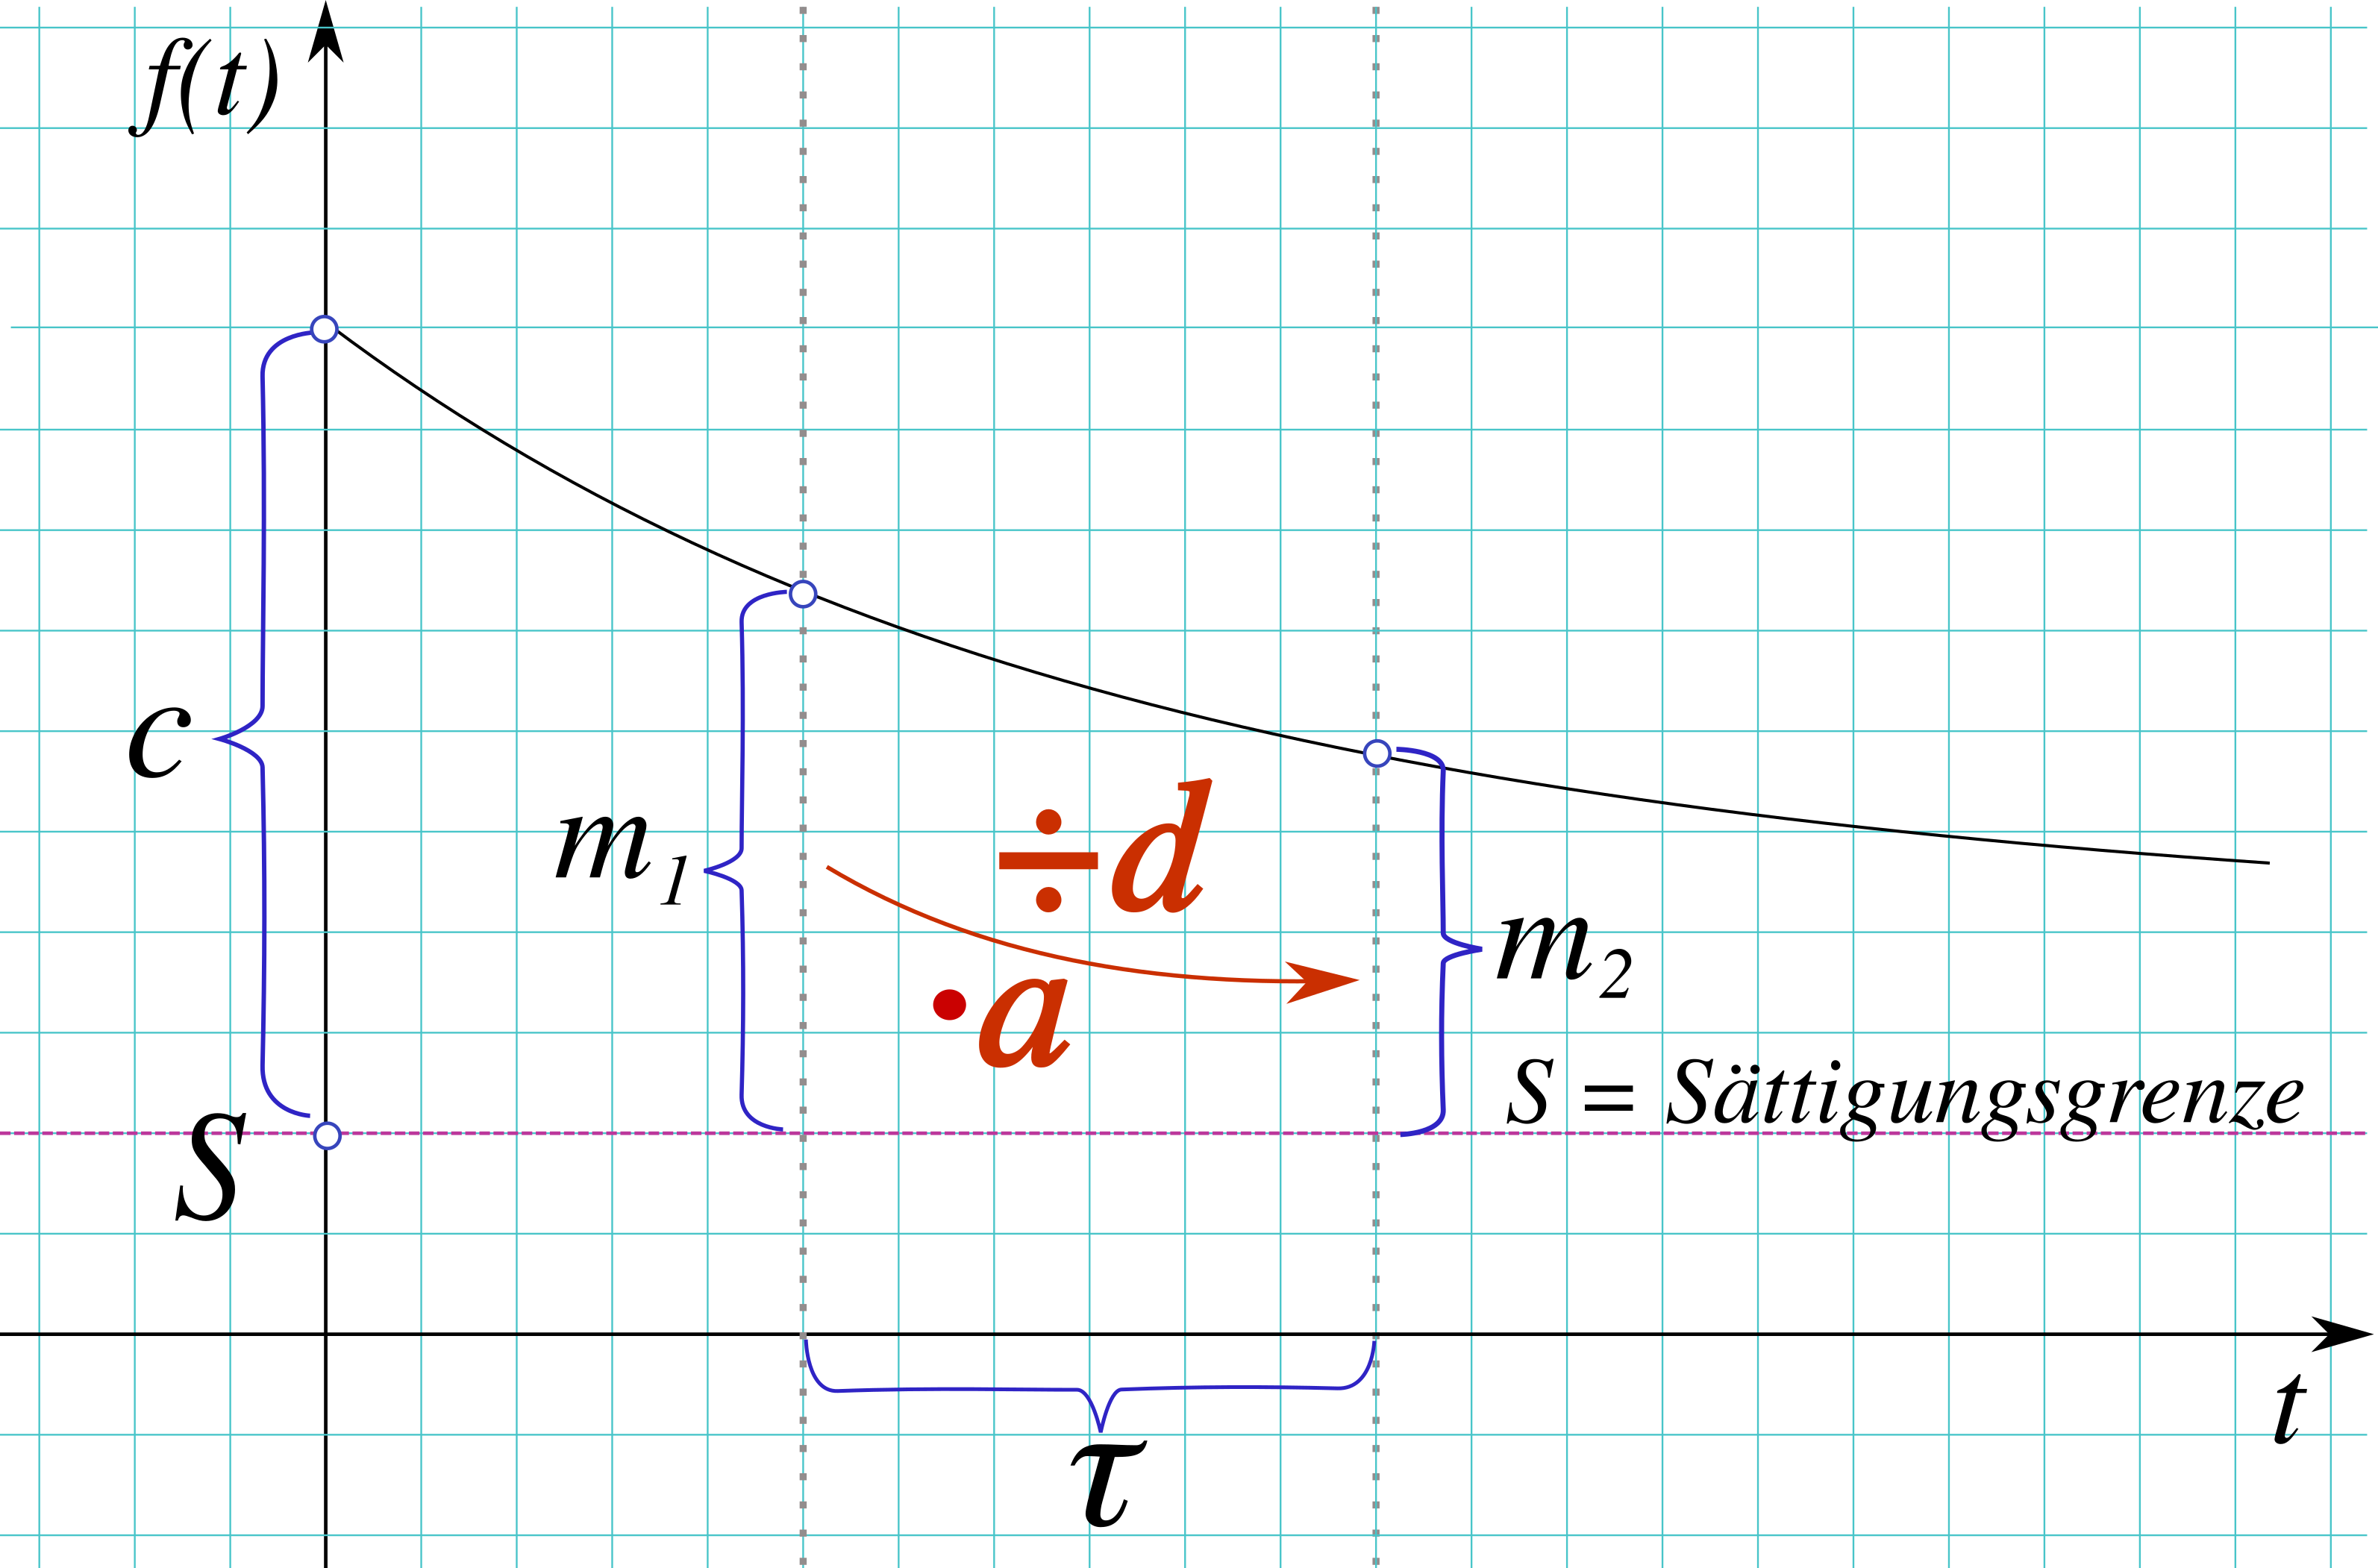
\includegraphics[width=13cm]{allg/funktionen/img/saettigung/saettigungskurveDown.png}}
\end{center}

Die Grundform eines begrenzten Zerfalls ist ein normaler
exponentieller Zerfall ($y=a^{t}$, $0<a<1$), der in $y$-Richtung um eine Sättigungsgrenze $c$ verschoben ist:

\begin{definition}{beschränkter Zerfall}{}
$$f(t) = c + b\cdot{}a^{\frac{t}{\tau}}$$
\end{definition}

Dabei ist:
\begin{itemize}
  \item $c+b = f(0) = y$-Achsenabschnitt = Startwert
	\item $c$: Die Sättigungsgrenze\index{Sättigungsgrenze} (Sättigungswert). Dies ist die Annäherungskonstante oder der \textbf{Asymtote}nwert\index{Asymptote}: Tiefer kann die Funktion nicht fallen.

	\item $m$:
    Sättigungs\textbf{differenz}\index{Sättigungsdifferenz}\index{Differenz!zur
      Sättigung}. Wie viel fehlt, bis zur
    Sättigungsgrenze: $m = f(t) - c$. Die Sättigungs\textbf{differenz} nimmt exponentiell ab.
	\item $b$: Die \textbf{Abweichung} zu $c$ zum Zeitpunkt $t=0$. Der
    Anfangswert ist somit $f(0) = c + b$; mit anderen Worten: $b$ ist das
    \textbf{Sättigungsdifferenz} zum Zeitpunkt $t_0 = 0$.
	\item $\tau$: Die Zeit zwischen zwei typischen Beobachtungszeitpunkten wird
    mit $\tau$ («tau») bezeichnet.
    \item $a=\frac{m}{b}=\frac{f(\tau)-c}{f(0)-c}$: Der Faktor der Veränderung der
      Sättigungdifferenz.
\end{itemize}

\subsection*{Aufgaben}
\GESOAadB{359}{35. (Kuchen) und 36. (Ovomaltine)}
\GESO{\aufgabenfarbe{Kompendium S. 33 Kap. 3.4.2 Aufg. 48 (Achtung: Das
  Kompendium verwendet andere Buchstaben: Das dortige $a$ ist unser $b$.)}}

\newpage


\subsection{Sättigung (begrenztes
  Wachstum)}\index{Sättigung}\index{begrenztes Wachstum}\index{Wachstum!begrenztes}
\subsubsection{Einstiegsbeispiel 1: Eistee wärmen}
Das Aufwärmen von Eistee von $5\degre$ Kühlschranktemperatur auf $20\degre$ Zimmertemperatur ist ein klassisches «Begrenztes Wachstum» (mit gespiegelter Exponentialfunktion).

\TNT{5.2}{Skizze}

\subsubsection{Einstiegsbeispiel 2: Batterie laden}
\begin{center}
\raisebox{-1cm}{
\includegraphics[width=8cm]{allg/funktionen/img/saettigung/batterien.png}}
\end{center}

Eine 9V-Batterie ist etwas mehr als zur Hälfte entladen und enthält nun eine
Restspannung von 4V.

Wenn wir 9V an die Batterie anlegen, so wird die Batterie geladen.

Die Batterie lädt sich umso rascher, je \textit{leerer} sie ist.

Die Batterie lädt sich umso langsamer, je \textit{voller} sie ist.


\newpage

\subsubsection{Allgemeine Form von Sättigungsprozessen}

\begin{center}
\raisebox{-1cm}{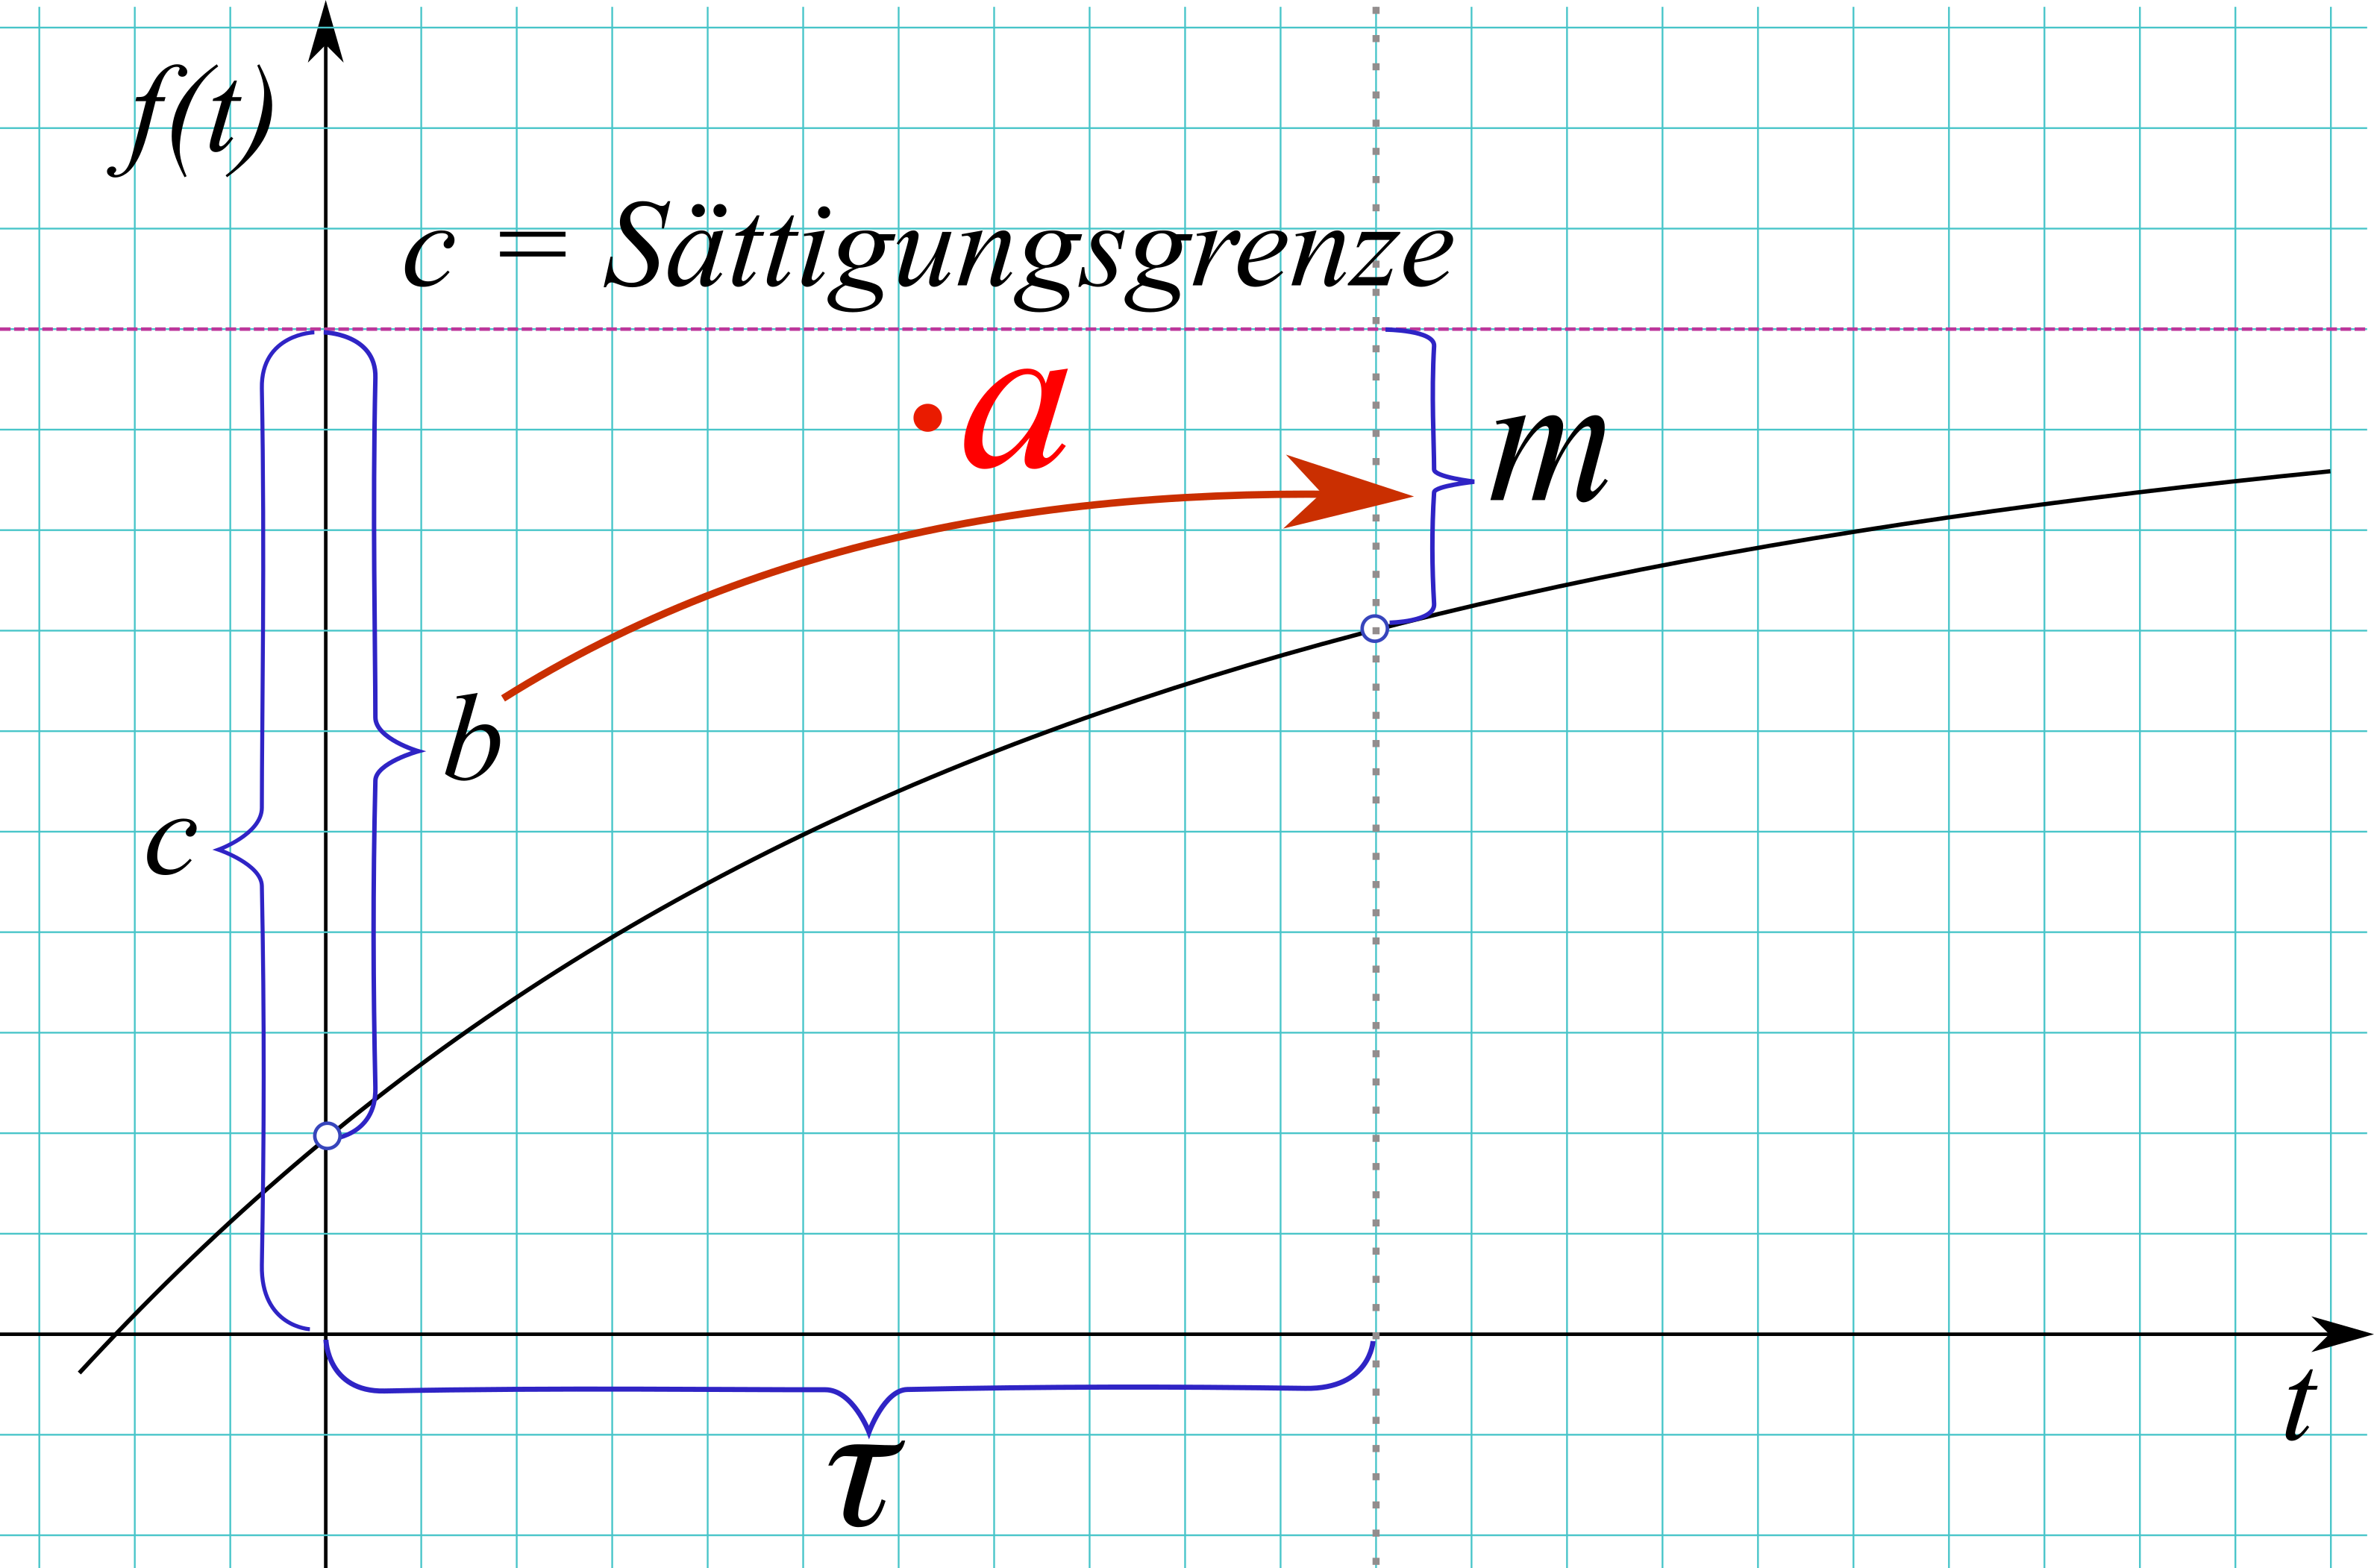
\includegraphics[width=13cm]{allg/funktionen/img/saettigung/saettigungskurve.png}}
\end{center}

Die Grundform des begrenzten Wachstums ist ein exponentieller Zerfall\totalref{zerfallsfunktion},
der an der $x$-Achse gespiegelt und in $y$-Richtung
verschoben ist:

\begin{definition}{Sättigung}{}
$$f(t) =c - b\cdot{} a^{\frac{t}{\tau}}$$
\end{definition}

Die Variable haben die folgenden Bedeutungen:

\begin{itemize}
	\item $c$: Sättigungsgrenze. Dies ist die Annäherungskonstante oder der Asymtotenwert. Höher kann die Funktion nicht steigen.

	\item $m$ ist die
    Sättigungsdifferenz\index{Sättigungsdifferenz}\index{Differenz!zur
    Sättigung}. Wie viel fehlt, bis zur
    Sättigungsgrenze: $m = c - f(t)$. Auch hier nimmt die Sättigungs\textbf{differenz} exponentiell ab.
	\item $b$: Die Abweichung des Funktionsgraphen zu $S$ zum Zeitpunkt $t=0$. Der
    Anfangswert ist somit $f(0) = c - b$.
	\item $\tau$: Die Zeit zwischen zwei typischen
    Beobachtungszeitpunkten.
\item $a=\frac{m}{b}=\frac{c-f(\tau)}{c-f(0)}$ Faktor der Veränderung
  der Sättigungsdifferenz.
\end{itemize}


\subsubsection{Bemerkungen}
\begin{bemerkung}{}{}
  Für die Sättigungsdifferenz gilt:

\TNT{4}{$$m = m(t) = c - f(t) = c - \left(c-b\cdot{}a^{\frac{t}{\tau}}\right) = + b\cdot{}a^{\frac{t}{\tau}}$$

und somit:

$$m_0 = m(0) = b\cdot{}a^0 = b$$}%% END TNT
\end{bemerkung}

\TRAINER{ Bemerkung (Trainer/mündlich):
  
Das $a$ kann aus zwei \textbf{beliebigen} Sättigungsdifferenz-Werten berechnet werden (die um die
Zeitdifferenz $\tau$ auseinander liegen):
$$\frac{m_2}{m_1} = \frac{b\cdot{}a^{\frac{t_2}{\tau}}}{b\cdot{}
  a^{\frac{t_1}{\tau}}} = a^{\frac{t_2}{\tau}} : a^{\frac{t_1}{\tau}} =
a^{\frac{t_2-t_1}{\tau}} = a^{\frac{\tau}{\tau}} = a$$%% 
}%% END Trainer


\begin{bemerkung}{}{}
Meistens ist $m_0$ zum Zeitpunkt $t=0$ bekannt und somit ist $b=m_0$. Es reicht, die Messung zum Zeitpunkt $t_0$ und zu einem weiteren Zeitpunkt durchzuführen. Wenn zusätzlich die Sättigungsgrenze $c$ bekannt ist, kann die Funktion $f$ komplett bestimmt werden.
\end{bemerkung} 

\newpage

\subsection{Referenzaufgaben}

\subsubsection{Berechnung am Batterie-Beispiel}\index{Batterie}
Eine Batterie weist zum Zeitpunkt $t_0$ vier Volt auf. Nach sechs Stunden am Ladegerät zeigt die Messung sieben Volt. Wir wissen, dass die Sättigungsgrenze (Ladespannung) bei neun Volt liegt.

Zeichnen Sie die gegebenen Größen in ein Koordinatensystem ein und markieren Sie bei neun Volt eine horizontale Beschränkungslinie (\zB 1V = 1 Häus'chen in $y$-Richtung; 1h = 1 Häus'chen in $x$-Richtung).

\noTRAINER{\mmPapier{8.8}}
\TRAINER{\bbwCenterGraphic{15cm}{allg/funktionen/img/saettigung/batterieFct.png}}

\textbf{Frage 1}: Wie lautet die Formel $f(t) = ...$ der Sättigungskurve?

\noTRAINER{$c = ..........................$}
\TRAINER{$c = \textrm{ Sättigungsgrenze } = 9 [\textrm{V}]$}

\noTRAINER{$b = ..........................$}
\TRAINER{$b = m_0 = c-f(0) = 9 - 4 = 5$}

\noTRAINER{$m =  ..........................$}
\TRAINER{$m = m_1 = c-f(\tau) = 9 - 7 = 2$}

\noTRAINER{$a = .........................$}
\TRAINER{$a=\frac{m}{b} = \frac{m_1}{m_0} = \frac{2}{5}$}

\noTRAINER{$\tau = .........................$}
\TRAINER{$\tau = 6$ ($e_x$ = eine Stunde)}


\noTRAINER{$f(t) = c - b\cdot{}a^{\frac{t}{\tau}} = ..... - .....\cdot{}(.....)^{\frac{-t}{.....}}$}
\TRAINER{$f(t) = c - b\cdot{}a^{\frac{t}{\tau}} = 9 - 5\cdot{}(\frac{2}{5})^{\frac{t}{6}}$}

\TRAINER{Die Kontrollen für $t=0$ und $t=6$ sind mit dem Stehenlassen von $a$ als Bruch nun sehr einfach.}
\newpage

\textbf{Frage 2}: Wann wird die Batterie zu 99\% geladen sein?

\TNT{6.4}{99\% von 9V = 8.91 V

  Somit ist $t$ gesucht mit $f(t) = 9 - 5\cdot{}(9.4)^{\frac{t}{6}} = 8.91$

  (beidseitig -9 und Vorzeichen drehen und dann durch 5 teilen, so folgt...)

  $$(0.4)^{\frac{t}{6}} = 0.09 : 5 = 0.018$$

  Definition Logarithmus:

  $$\frac{t}6 = \log_{0.4}(0.018) \approx 26.3 $$

  Nach ca. 26 - 27 Stunden ist die Batterie zu 99\% geladen.
}
\newpage

\subsubsection{Referenzaufgabe Sättigung: Pneu}\index{Reifen}\index{Pneu}

Ein Reifen (Pneu) ist anfänglich ganz leer und enthält «nur» 1 at, nämlich den
Druck der Umgebung. 

Der Reifen wird aufgepumpt mit einer Druckpumpe, die maximal 2 at
(1 at = atmosphärischer Druck = technische Atmosphäre) leisten
kann. Mit 2 at ist hier gemeint: 2 at mehr als der
Umgebungsdruck. Somit könnte der Pneu bis auf maximal 3 at aufgepumpt
werden (= Sättigungsgrenze).

Um den Reifen optimal zu füllen, wird er auf 2 at aufgepumpt (1 at
über dem Umgebungsluftdruck).

Die Pumpe schafft in den ersten 10 Sekunden den Druck von 1 at auf 1.2
at (= 0.2 at über Normaldruck) aufzupumpen.

Nach wie vielen Sekunden muss gestoppt werden, damit der Reifen
optimal gepumpt ist?

\TNT{8}{Die Sättigungsdifferenz schwindet von $m_1=3-1=2$ bis $m_2=3-1.2=1.8$
innerhalb der ersten $10s = \tau$. Die Sättigungsgrenze liegt bei
$S=3$. Unsere (Exponential)basis $a$ ist somit $1.8 / 2$, was uns
liefert:
$$f(t) = 3 - 2\cdot{}\left(\frac{1.8}{2}\right)^\frac{t}{10}$$
Somit ist das Optimum bei $2 = 3-
2\cdot{}\left(\frac{1.8}{2}\right)^\frac{t}{10}$ erreicht, also bei
etwa 65.8 Sekunden.
}
\newpage

\subsubsection{Referenzaufgabe: Ritter
  Nimmersatt}\index{Nimmersatt!Ritter}\index{Ritter Nimmersatt}
Ritter Nimmersatt ist nimmer satt. Erst bei einer Magenfülle von
5 Litern stößt ihm alles wieder auf. Richtig wohlgenährt ist er
normalerweise erst bei einem Magen, der zu 4.5 Liter gefüllt ist.

Er beginnt das Festmahl bei Kunigundes Hochzeit mit einer Magenfülle
von 2 Litern\footnote{Darunter würde er echte Hungerschübe
  leiden!}. In der ersten Minute schafft er es, 3 dl Flüssigkeit oder Nahrung
in sich regelrecht hineinzustopfen. Danach nimmt sein Futtern
exponentiell ab (bis zur Sättigungsgrenze von 5 Litern, die er
hoffentlich nicht erreicht).

Nach wie vielen Minuten ist er so richtig gesättigt; m.\,a.\,W. wann
hat er besagte 4.5 Liter im Magen\footnote{Der Moment ist gekommen, wo
  die Wachen den Ritter Nimmersatt vorsorglich unter irgend einem Vorwand aus der Burg schaffen sollten.}?

\TNT{8}{
  $c = 5$, $b = m_0 = 5-2=3$, $m=m_1= 5-2.3=2.7$, $\tau = 1$, $a=\frac{2.7}{3} = 0.9$ und somit:
  $$f(t) = 4.5 = 5 - 3\cdot{}\left(\frac{2.7}{3}\right)^t$$
Und so ist er nach 17 Minuten so richtig satt.\vspace{52mm}}


\GESO{\subsection*{Aufgaben}}
\GESOAadB{358}{34. (Eistee)}
\GESO{\aufgabenfarbe{Kompendium S. 32ff Kap. 3.4.2 Aufg. 49-51 (Bem.: Das
  Kompendium gibt die Funktionsterme bereits an und verwendet als
  Basis die Eulersche Konstante $e\approx{} 2.71828$)}}
\newpage

\subsection{Zusammenfassung der Prozesse}
\vspace{8mm}
\begin{center}\textbf{Wachstum und Zerfall}\end{center}

\TNT{6}{\bbwCenterGraphic{18cm}{allg/funktionen/img/zusammenfassung_exp/wachstum_zerfall.png}}%% END TNT

\vspace{8mm}
\begin{center}\textbf{Sättigung}\end{center}

\TNT{6}{\bbwCenterGraphic{18cm}{allg/funktionen/img/zusammenfassung_exp/saettigung.png}}%% END TNT

\TRAINER{Hier ist Platz für das Video/die Videos zur den getanzten
  Funktionen (S. OLAT/Wiki).}
\newpage
%%
%% 2019 07 04 Ph. G. Freimann
%%

\section{Logarithmusfunktionen}\index{Funktionen!Logarithmus}\index{Logarithmusfunktionen}
\sectuntertitel{$e^x$}
%%%%%%%%%%%%%%%%%%%%%%%%%%%%%%%%%%%%%%%%%%%%%%%%%%%%%%%%%%%%%%%%%%%%%%%%%%%%%%%%%
\subsection*{Lernziele}

\begin{itemize}
\item Umkehrung der Exponentialfunktion
\item Nullstellen, Definitionsbereich
\end{itemize}

\TALS{(\cite{frommenwiler17alg} S.227 (Kap. 3.11))}
\GESO{(\cite{marthaler21}       S.329 (Kap. 19.2))}


\subsection{Definition}
Die Funktion $f(x): x \mapsto y = log(x)$ ist eine
Logarithmusfunktion.

\subsubsection{Umkehurng der
  Exponentialfunktion}\index{Umkehrfunktion!der Exponentialfunktion}

Skizzieren Sie $f(x) = 2^x$ und $g(x) = \log_2(x)$ ins selbe
Koordinatensystem und markieren Sie die charakteristischen Punkte. Was
ändert sich, wenn Sie bei $f$ und $g$ statt der Zahl $2$ die Zahl $3$
verwenden?

\TNTeop{
  Bei der Exponentialfunktion $f$ ist 1 der $y$-Achsenabschnitt. Bei
  $g$ ist 1 die Nullstelle.

  $f$ hat keinen Funktionswert $\le 0$ während der Definitionsbereich
  von $g$ auch nur Zahlen größer als $0$ sein können.

  Die beiden Funktionen $f$ und $g$ sind sich gegenseitig
  Umkehrfunktionen und somit das Spiegelbild an der Diagonalen $x=y$
  im Koordinatensystem.

  
}
\newpage


\subsection*{Aufgaben}
\TALSAadB{227ff}{856-879}
  \olatLinkTALSStrukturaufgabenSPF{Basiskenntnisse Funktionen Teil
    1}{4}{3.}
  \olatLinkTALSStrukturaufgabenSPF{Basiskenntnisse Funktionen Teil
    2}{15}{53. und 54.}


\GESOAadB{340ff}{42-51}
\newpage


%%%%%%%%%%%%%%%%%%%%%%%%%%%%%%%%%%%%%%%%%%%%%%%%%%%%%%%%%%%%%%%%%%%%%%%%%%%
%%
%% 26. März 2013: Philipp Gressly Freimann
%%
\appendix

\section{Anhang}

%
% Griechisches Alphabet bei TALS Trigo anfügen als Anhang
%

\subsection{Das griechische Alphabet}
\sectuntertitel{${\color{green} 33\omega}$-Witz: Ist schon gebratenes $\lambda$? Nein, das $\varphi$ ist noch $\varrho$.}

\vspace{4mm}

%% Diejenigen Großbuchstaben, welche im Deutsch gleich sind (A, B),
% werden im mathematischen Formelsatz auch kursiv geschrieben.

\begin{tabular}{ll|ll}
  
  $\alpha \textrm{A}$                & «alfa»    & $\nu \textrm{N}$            & «nüü»       \\
  $\beta \textrm{B}$                 & «beta»    & $\xi \Xi$                   & «gsii»      \\
  $\gamma \Gamma$                    & «gamma»   & $\textrm{o} \textrm{O}$     & «oh-micron» \\    
  $\delta \Delta$                    & «delta»   & $\pi \Pi$                   & «pi»        \\    
  $\epsilon \varepsilon \textrm{E}$  & «epsilon» & $\rho \varrho \textrm{P}$   & «rho»       \\    
  $\zeta \textrm{Z}$                 & «zeta»    & $\sigma \Sigma$             & «sigma»     \\    
  $\eta \textrm{H}$                  & «eta»     & $\tau \textrm{T}$           & «tau»       \\    
  $\theta \vartheta \Theta$          & «theta»   & $\upsilon \Upsilon$         & «üpsilon»   \\    
  $\iota \textrm{I}$                 & «iota»    & $\phi \varphi \Phi$         & «phii»      \\    
  $\kappa \textrm{K}$                & «kappa»   & $\chi \textrm{X}$           & «chii»      \\    
  $\lambda \Lambda$                  & «lambda»  & $\psi \Psi$                 & «psii»      \\    
  $\mu \textrm{M}$                   & «müü»     & $\omega \Omega$             & «Oh! Mega!» \\    
\end{tabular}

\textit{\textbf{Legende}: Sind drei griechische Buchstaben angegeben, so bezeichnen die
ersten beiden zwei verschiedene Varianten der Kleinschreibung.}
\newpage

%%\sectuntertitel{Was ich sonst noch alles sagen wollte.}
%%%%%%%%%%%%%%%%%%%%%%%%%%%%%%%%%%%%%%%%%%%%%%%%%%%%%%%%%%%%%%%%%%%%%%%%%%%%%%%%%


%%%%%%%%%%%%%%%%%%%%%%%%%%%%%%%%%%%%%%%%%%%%%%%%%%%%%%%%%%%%%%%%%%%%%%%%%%%

%%\linkVerzeichnis{}%%

%%%%%%%%%%%%%%%%%%%%%%%%%%%%%%%%%%%%%%%%%%%%%%%%%%%%%%%%%%%%%%%%%%%%%%%%%%%
%\newpage\mbox{}
%\blankOddPage{}%
%\include{texlife-bibtex-extra}

\bibliography{bibAll.bib}{}\label{literatur}

\printindex
%%%%%%%%%%%%%%%%%%%%%%%%%%%%%%%%%%%%%%%%%%%%%%%%%%%%%%%%%%%%%%%%%%%%%%%%%%%
 
\end{document}
